
Для того, чтобы разобраться в том, как формируются экспериментальные
двухкристальные КДО, необходимо построить спектрально-угловое распределение пучка
в соответствии с реальной схемой эксперимента (рис. \ref{ris:double_crystal_schem_lamtet_a}).

\begin{eqnarray} \label{eq:doudle_spectra_angle_map}
  P(\theta,\vartheta,\lambda) = g_{\lambda}(\lambda)g_{\vartheta}(\vartheta) P_M \left(\vartheta - \frac{\lambda - \lambda_1}{\lambda_1}\tan(\theta_B) \right) \cdot \nonumber \\
   P_S \left(\theta + \vartheta - \frac{\lambda - \lambda_1}{\lambda_1}\tan(\theta_B)\right).
 \end{eqnarray}

Выражение (\ref{eq:doudle_spectra_angle_map}) определяет спектрально-угловое распределение излучения после прохождения двух кристаллов с
коэффициентами отражения  $P_M$ (монохроматор) и $P_S$ (образец), причем последний в процессе сканирования подвергается отстройки от точного угла Брэгга
 (рис. \ref{ris:double_crystal_schem_lamtet_b}).

\begin{figure}[H]
  \centering
  \subfloat[]{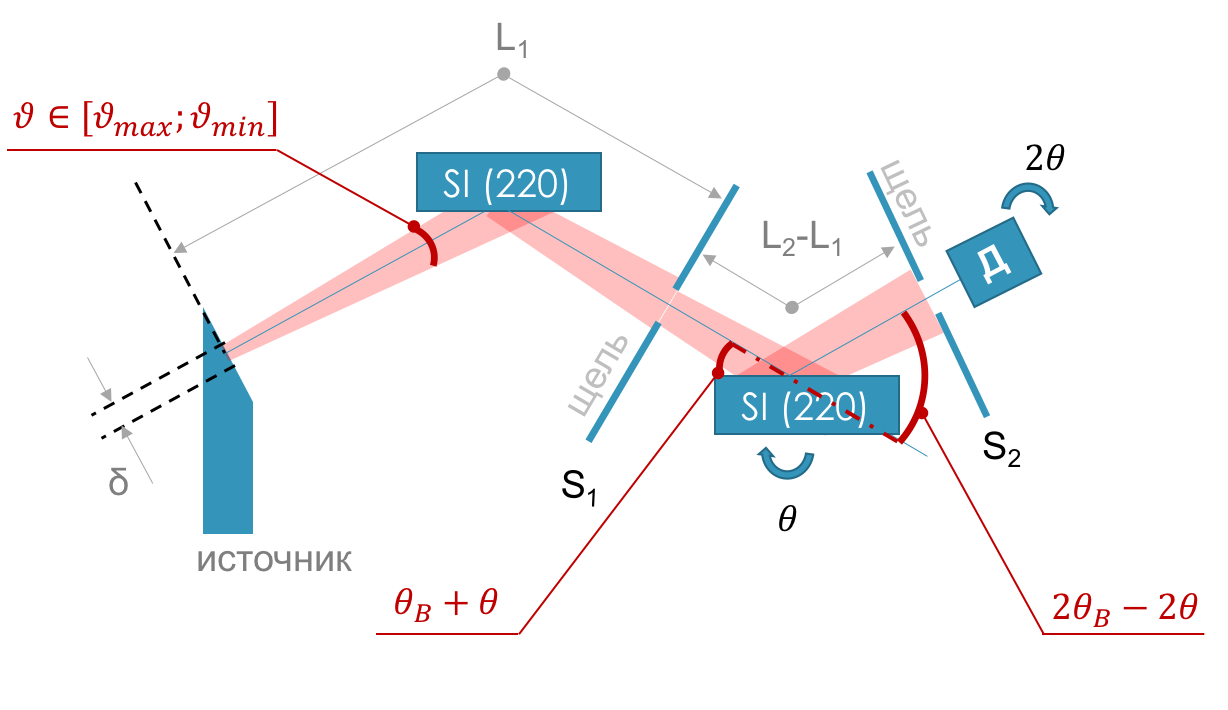
\includegraphics[width=0.5\textwidth]{images/double_crystal_schem.png}\label{ris:double_crystal_schem_lamtet_a}}
  \hfill
  \subfloat[]{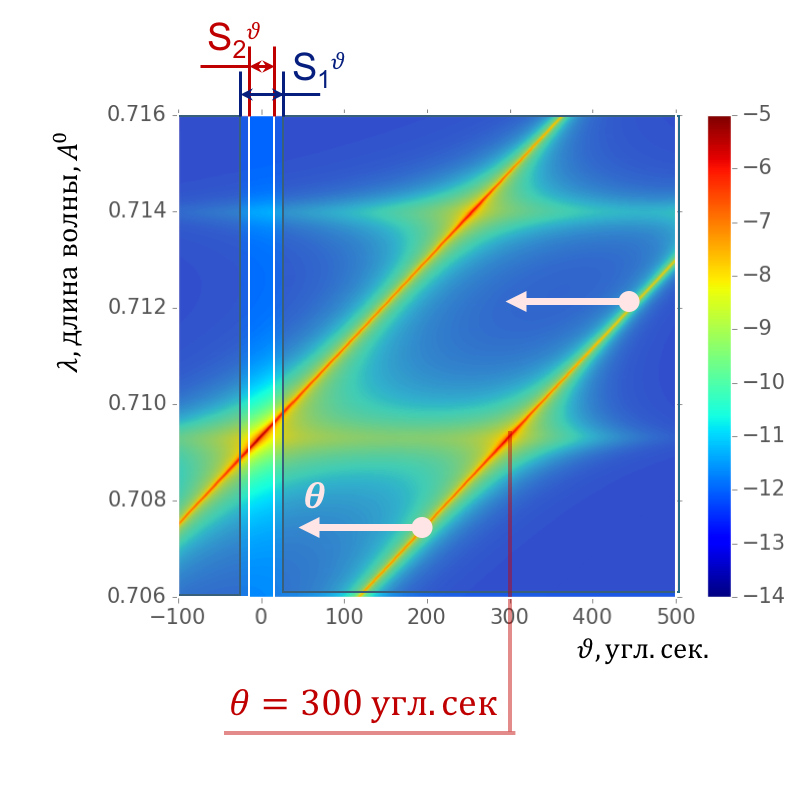
\includegraphics[width=0.45\textwidth]{images/double_crystal_schem_lamtet.png} \label{ris:double_crystal_schem_lamtet_b}}

  \caption{Схема (a) и спектрально-угловое распределение излучения (b) после
  отражения расходящегося, полихромотического пучка рентгеновской трубки с $Mo$-анодом.
  Несмотря на то, что в экспериментальной схеме детектор с приемной
   щелью не статичны, на карте обе щели $S_1$ и $S_2$ неподвижны.
  Положение щелевых устройств обозначено синей и белой линиями
  вблизи $\vartheta = 0$ угл.сек. Отстройка кристалла-образца от
  точного брэгговского положения составляет 300 угл. сек. }
  \label{ris:double_crystal_schem_lamtet}
\end{figure}

Выражение (\ref{eq:doudle_spectra_angle_map}) не учитывает особенности влияния
 щелевых коллиматоров, о которых мы говорили в
разделе \ref{sec:slits_section}. С учетом того факта, что детектор не разделят
 энергетическую составляющую пучка, что приводит к необходимости интегрирования по $\lambda$.
Конечное выражение для описания двухкристальной КДО примет вид:

\begin{eqnarray} \label{eq:doudle_spectra_angle_map_on_detector}
  P_{double}(\theta) = \sum_{\lambda = -\infty}^{\infty}g_{\lambda}(\lambda)\cdot
  \sum_{\vartheta = \vartheta_{s1}}^{\vartheta_{s2}} g_{\vartheta}(\vartheta) g_{S}(\vartheta) \cdot \nonumber \\
   P_M \left(\vartheta - \frac{\lambda - \lambda_1}{\lambda_1}\tan(\theta_B) \right) \cdot \nonumber \\
   P_S \left(\theta + \vartheta - \frac{\lambda - \lambda_1}{\lambda_1}\tan(\theta_B)\right),
 \end{eqnarray}
 \noindent
 где пределы суммирования определяются как $\vartheta_{s2} = - \vartheta_{s1} = \frac{\delta+S_1}{2L_1}$,
 $\delta$ - линейный размер источника.

 На рис. \ref{ris:double_crystal_form_kdo} изображен процесс формирования
 бездисперсионной КДО в процессе смещения справа налево наклонной линии отражения
 для кристалла-образца. В момент совпадения полос отражения монохроматора и образца
 на детекторе фиксируется максимальная интенсивность.

 \begin{figure}[H]
   \centering
   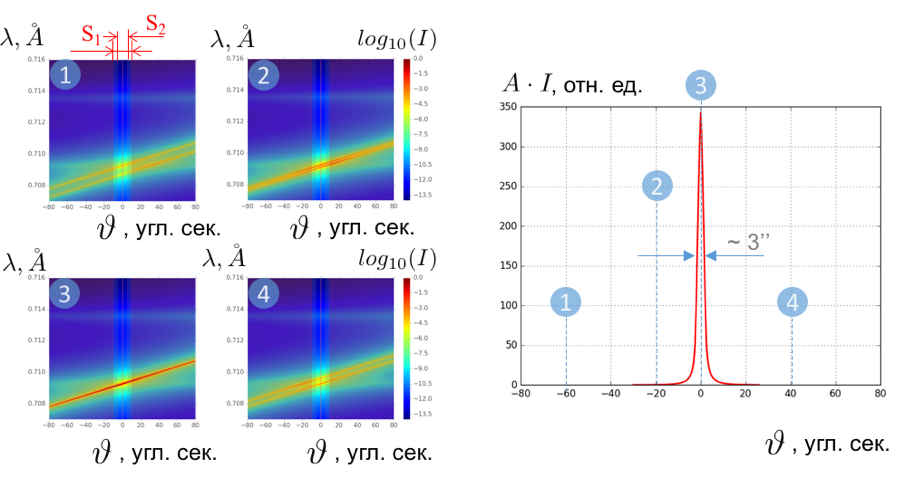
\includegraphics[width=1\textwidth]{images/double_crystal_form_kdo.png}
   \caption{Формирование двухкристальной кривой дифракционного отражения
    ($\theta - 2\theta$ - cканирование) для кристаллов Si(220)
   $\theta_B^M = \theta_B^S = 10.6^o$  $MoK_{\alpha}$ - излучения}
   \label{ris:double_crystal_form_kdo}
 \end{figure}

В случае, если схема дисперсионная т.е. углол Брэгга кристалла - образца отличен от угла Брэгга кристалла-монохроматора,
наблюдается уширения двухкристальных кривых, что можно наглядно наблюдать
на спектрально-угловой карте (рис. \ref{ris:double_crystal_form_kdo_dissp}).
 \begin{figure}[H]
   \centering
   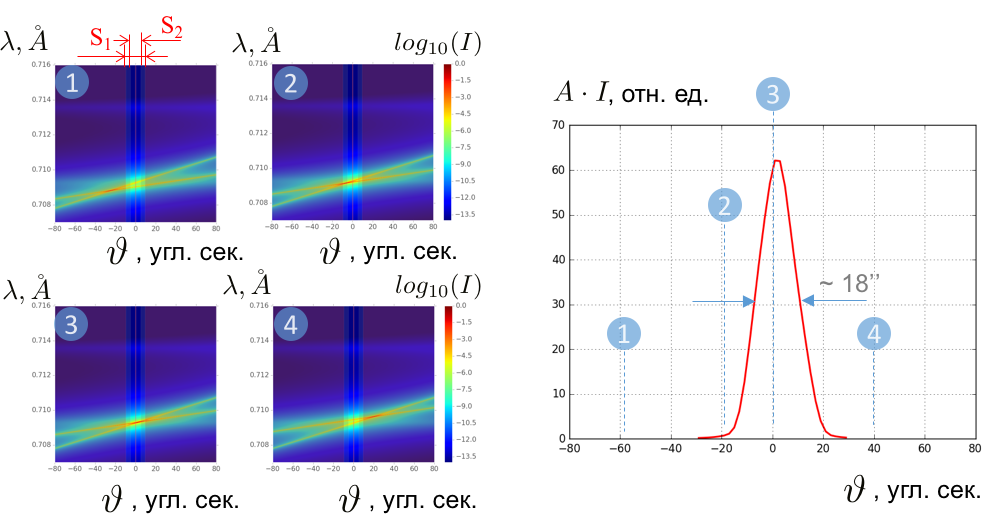
\includegraphics[width=1\textwidth]{images/double_crystal_form_kdo_dissp.png}
   \caption{Формирование двухкристальной кривой дифракционного отражения
   ($\theta - 2\theta$ - cканирование) в дисперсионной схеме для отражений Si(220) и Si(440)
   ( $\theta_B^M = 10.6^o$, $\theta_B^S = 21.6^o$)  $MoK_{\alpha}$ - излучения}
   \label{ris:double_crystal_form_kdo_dissp}
 \end{figure}
